\documentclass{article}

\usepackage[letterpaper,top=2cm,bottom=2cm,left=2cm,right=2cm,marginparwidth=1.75cm]{geometry}

\usepackage{amsmath}
\usepackage{multirow}
\usepackage{graphicx}
\usepackage{array}
\usepackage{titlesec}
\usepackage{lipsum}
\usepackage{mwe}
\usepackage[parfill]{parskip}
\usepackage[colorlinks=true, allcolors=blue]{hyperref}

\pdfpagewidth=8.5in
\pdfpageheight=11in


\def\tricolfig#1{\includegraphics[width=2.2in]{#1}}
\def\triplecolfig#1{\includegraphics[width=0.32\textwidth]{#1}}
\def\smallcolfig#1{\includegraphics[width=2.0in]{#1}}
\def\smallercolfig#1{\includegraphics[width=0.75\columnwidth]{#1}}
\def\mediumcolfig#1{\includegraphics[width=0.9\columnwidth]{#1}}
\def\colfig#1{\includegraphics[width=\columnwidth]{#1}}
\def\pagefig#1{\includegraphics[width=0.75\textwidth]{#1}}
\def\suspcolfig#1{\includegraphics[width=2.0in]{#1}}
\def\perfcolfig#1{\smallercolfig{#1}}



\def\crcd{compiler-runtime co-design}
\def\ALL{allocation}
\def\DALL{deallocation}
\def\ALLS{allocations}
\def\DALLS{deallocations}
\def\DWS{dynamic memory working set size}
\def\SIZE{allocation size}
\def\SIZES{allocation sizes}



\title{Compiler and Runtime Support for Functions-as-a-Service (FaaS)}
\date{}
\author{Souradip Ghosh, 15-849, Fall 2021}

\begin{document}
\maketitle

\section{Abstract}
Functions-as-a-Service (FaaS) are rapidly growing in popularity and 
complexity among cloud service provides as users look to take 
advantage of cloud resources on-demand and focus on computation
at a finer grain. FaaS instances are characteristically short-lived
and often dominated by communication and cold-start overheads compared
to typical monolithic applications. At the same time, FaaS instances
are requiring more resources, especially memory, to operate. Although
many works have approached these issues with scheduling optimizations,
hardware accelerators, and other techniques, very few have examined
\textit{compiler} support and \textit{\crcd} for FaaS. This paper presents 
a \crcd\ consisting of static analyses, profiling, and a custom memory 
allocator controlled by the compiler and runtime to better understand 
and optimize \textit{dynamic memory usage} for small FaaS workloads.

\section{Design}
The design of the system consists of three major components : 1) a \textit{profiler},
2) \textit{static analyses} in the compiler, and 3) a \textit{custom memory allocator}
that is \textit{designed and optimized with FaaS characteristics in mind}. The first and third components consist 
of compiler instrumentation coupled with an integrated runtime. All analyses and 
transformations operate on the \textit{intermediate representation} (IR) of the compiler, 
where standard compiler optimizations are performed. These components are described in 
the following subsections in detail. 

\begin{figure}[htp]
    \centerline{\pagefig{figs/sys.pdf}}
    \caption{System overview and compilation pipeline. }  
	\label{fig:sys}
\end{figure}

An overview of the system and compilation pipeline is show in Figure~\ref{fig:sys}. The 
first pass over an example workload (\texttt{app.c}) consists of static analyses and 
profiling. The second pass over \texttt{app.c} instruments the program with the custom
allocator using the results from the static analyses (and optionally the profiler). This 
custom allocator replaces standard dynamic \ALLS\ and \DALLS\ in \texttt{app.c}, and it is
the \textit{crux} of optimization for dynamic memory usage in FaaS workloads in this system. The
outputs from this compilation pipeline include an instrumented application (\texttt{app.exe})
and statistics about \DWS\ (total size for all dynamic \ALLS).

\subsection{Profiler} \label{prof}
The profiler has the goal of understanding information about dynamic memory \ALLS\ and 
\DALLS\ during execution (for instance, the number of \ALLS\, \DWS\, common \ALL\ 
sizes, etc.) as well as typical information about critical paths or the "hotness" of functions and
loops at runtime that is often use to aid optimization. Using this data, the profiler can inform the compiler during 
instrumentation in the second pass over the application (see \ref{ca}). It can also 
inform the user with a better estimate of memory usage for a future FaaS instance or 
function invocation.

The profiler tracks all \ALLS\ and \DALLS\ of some workload, $W$, at runtime. This is 
accomplished by using the compiler to instrument all explicit dynamic memory \ALL\ and \DALL\ function 
calls in the IR for $W$ with \textit{callback} functions to a profiler runtime.
Two callbacks, \texttt{TrackAllocation(ptr, size)} and \texttt{TrackDeallocation(ptr)}, are 
sufficient to achieve all tracking. \texttt{TrackAllocation} takes a pointer to an allocation (\texttt{ptr}) and 
the size of the allocation (\texttt{size}) as inputs and records the pair in a table in the 
profiler's runtime. \texttt{TrackDeallocation} simply takes a pointer to an allocation (\texttt{ptr}) as
input and removes the entry from the profiler runtime's table. An example of this 
instrumentation is shown in Figure~\ref{fig:pins}.

\begin{figure}
    \centering
    \begin{minipage}{0.45\textwidth}
        \centering
        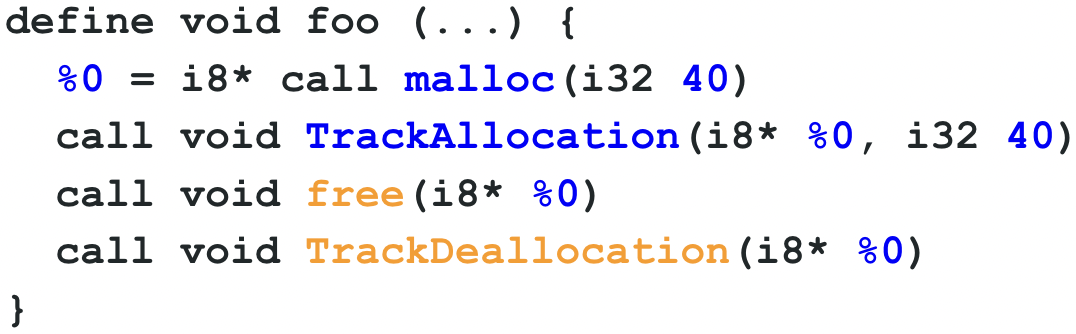
\includegraphics[width=0.9\textwidth]{figs/pins.png} 
        \caption{Example compiler instrumentation for profiler callbacks in the 
        context of simplified LLVM IR and \textit{libc} \texttt{malloc}
        and \texttt{free}}  
	    \label{fig:pins}
    \end{minipage}\hfill
    \begin{minipage}{0.45\textwidth}
        \centering
        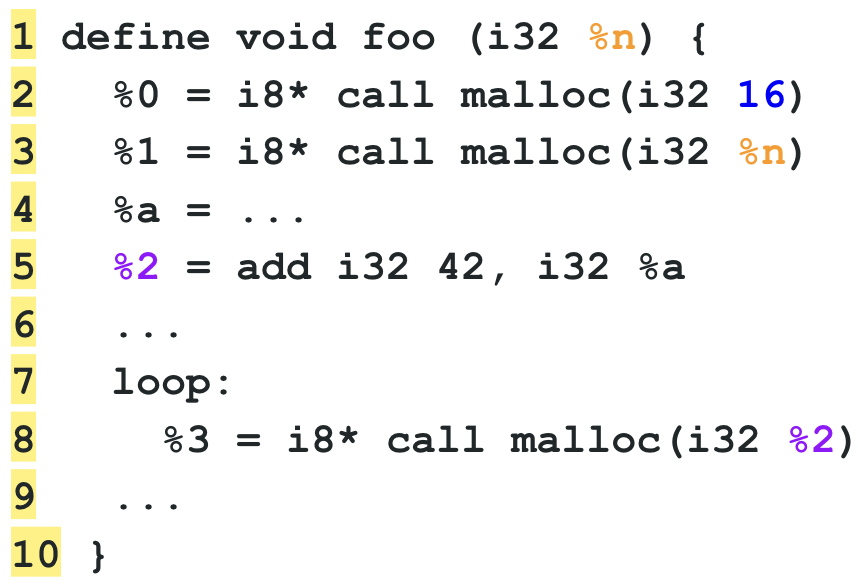
\includegraphics[width=0.70\textwidth]{figs/sizes.png} 
        \caption{Example allocations that the static analysis can target in the 
        context of simplified LLVM IR and \textit{libc} \texttt{malloc}}  
	    \label{fig:sizes}
    \end{minipage}\hfill
\end{figure}

While $W$ runs, the profiler tracks each change to the \DWS\ over its entire execution 
whenever a callback is invoked. Using this information, the profiler calculates maximum 
and average \DWS\ for $W$ and outputs the data to the user and to the compiler for future 
use. All profiler information can be optionally used by the custom allocator component of
the \crcd\ (see \ref{ca}).

\subsection{Static Analyses} \label{sa}
The system also supports static analyses of \ALLS\ and \DALLS\ in the IR for workload $W$. 
In particular, the compiler analyzes 1) \ALL\ sizes for all \ALLS\ , 2) loops to unroll 
and functions to inline so that 1) is more feasible to analyze, and 3) uses of \ALL\ and 
\DALLS . All analyses informs the compiler about analyzable static allocations. 

The first analysis is especially important to identify \ALL\ and \DALL\ candidates that
can be replaced with the custom allocator. At a high level, the "easier it is to deduce"
the allocation \textit{size} for each \ALL\, the easier it is to replace the \ALL\ with one
of the methods from the custom alloactor (see \ref{ca} for details).

An "easy-to-deduce" or \textit{statically analyzable} \SIZE\ is one that is 
simply a constant integer. All other \SIZES\ are \textit{analyzable with
assistance}, where the size can apparently be deduced during runtime. These 
categories are mutually exclusive. The compiler records all statically analyzable 
\SIZES . An example is shown in Line 2 of Figure~\ref{fig:sizes}.

Some \SIZES\ that are analyzable with assistance are worth recording, however. In
particular, if an \SIZE\ is dependent on function arguments, the function (and
its parent functions) can be continually inlined until the size is statically
analyzable. Consequently, the compiler marks functions that are candidates for
aggressive inlining (compared to a standard inliner in \texttt{-O3}). An example of
this is shown in Line 3 of Figure ~\ref{fig:sizes}. At an
extreme, aggressive inlining can reach a point where it may be beneficial to
inline the entry-point function of $W$. This is especially common in small 
FaaS workloads where \ALLS\ towards the beginning of the workload have \SIZES\
dependent on the inputs. Obviously, inlining the entry-point function is not 
possible, but we can borrow concepts from JIT compilation or binary translation
to possibly embed the inputs into the binary itself. This process can occur
right before $W$ is invoked in the FaaS instance. A subset of this system's compiler
can analyze and transform $W$ as necessary. This solution is theoretical and 
not applied in this work.

Additionally, \SIZES\ that exists in a loop and are dependent on loop-invariant
values are also recorded. Here, the loop itself can be aggressively unrolled and
the \ALLS\ can be merged or replaced with one of the methods from the custom 
allocator. It is also important that the size is dependent on a loop-invariant 
value, or else the compiler cannot affirmatively analyze multiples of the size or
determine an appropriate unroll factor (unrolling too much without knowledge of
the \SIZE\ may be sub-optimal). An example of this is shown in Line 8 of Figure ~\ref{fig:sizes}.

Finally, the compiler analyzes the uses of \ALLS , especially if they are used
in explicit \texttt{store} operations in the IR. An \ALL\ pointer that is stored
to an arbitrary memory location is an \textit{escape}, and it is very difficult
to analyze its value, lifetime, and size once it leaves the scope of its parent
function. Additionally, it is hard to manage \DALLS\ if pointer origins
cannot be deduced, which can be common with escaped \ALL\ pointers. All escapes
are recorded. All \ALLS\ and \DALLS\ that cannot be statically analyzed using
memory alias analysis (i.e "must alias" conditions) or def-use chains are conservatively flagged.

\subsection{Custom Allocator} \label{ca}
The final component of the system is a custom memory allocator, managed by both
the compiler and runtime and designed with consideration of FaaS characteristics.
In particular, the allocator aims to reduce raw \ALL\ and \DALL\ time, consolidate 
\ALLS\, and utilize compiler analysis to optimize dynamic memory overheads. 

The allocator primarly takes the static analyses (see \ref{sa})
as input to replace as many \ALLS\ and \DALLS\ with invocations to the allocator. If
an allocation is not selected as a candidate for any transformations, it is left unchanged.
First, \ALLS\ with statically analyzable \SIZES\ are prime candidates to be 
\textit{pre-allocated} because all the information needed to allocate is known at
compile-time. These \ALLS\ are placed into a \textit{compiler-directed memory pool} that is
allocated by the runtime in parallel to FaaS instance startup and before the entry-point function 
of the workload, $W$, begins. The size of the pool is the sum of all statically 
analyzable \SIZES\ of the selected \ALLS . As a result, the \ALL\ function calls are 
replaced by a load of a compiler-determined offset of the pool's base address.
An \ALL\ can only be selected for this transformation if it is not flagged by 
the escapes analysis (see the third analysis in \ref{sa}) \textit{and} the compiler 
can deduce the number of invocations of its parent function or of the allocation
itself (if it belongs to a loop, for instance). Otherwise, the data
in memory or the pointer itself may be overwritten accidentally. The latter condition
can be alleviated with aggressive inlining and function versioning. An example of 
this transformation is shown in Figure~\ref{fig:pool}. There are a number of 
benefits to this approach: 1) alleviating function call overheads, 2) enabling 
prefetching of allocation pointer address, and 3) hiding allocation overhead by performing 
it before $W$ even begins. This can boost performance and simplifies memory management
for FaaS instances. 

Allocations that have statically analyzable size but could not be transformed to
use the compiler-directed memory pool, can still be transformed to invoke other
methods of the allocator. We motivate this by a simple example: a node 
to a linked list is allocated during an irregular while loop. These \ALLS\ most
likely belong to the same static IR instruction, but are invoked many times with
the same \SIZE\ during the loop. Consequently, we transform these \ALLS\ to 
invoke an allocation callback from a fast \textit{bump allocator} that has a block size equal to the 
\SIZE . The callback, \texttt{AllocateFromBump(blk\_size)}, returns a pointer from the
runtime's bump allocator dedicated to a block size of \texttt{blk\_size}. The bump allocator
for \texttt{blk\_size} is initialized in parallel to FaaS instance startup via 
a compiler-injected callback, since \texttt{blk\_size} is already known at compile-time.
All bump allocators are stored by their block sizes in the runtime.

Finally, \ALLS\ that may be invoked many times (as in the example), but have 
variable-dependent \SIZES\ (i.e. the size is not a constant integer) are transformed to 
invoke a callback, \texttt{AllocateFromBumpWithRuntimeInit(blk\_size)}, that performs 
bump allocator initialization during runtime if the allocator for \texttt{blk\_size} is not
yet initialized. Allocations that fit the criteria for this transformation include ones
in loops with loop-invariant and variable-dependent \SIZES .

It is important to note that the profiler (see \ref{prof}) can aid these transformations.
For instance, identifying hot functions can expand the number of \ALLS\ that could
be transformed to invoke \texttt{AllocateFromBumpWithRuntimeInit}, since those static
\ALLS\ would be executed many times. Moreover, each bump allocator starts with a pool of 
a default number of of entries to allocate from before expanding to more pools. Using
profile information, the number of entries could be tuned for each specific bump allocator.

\begin{figure} [htp]
        \centering
        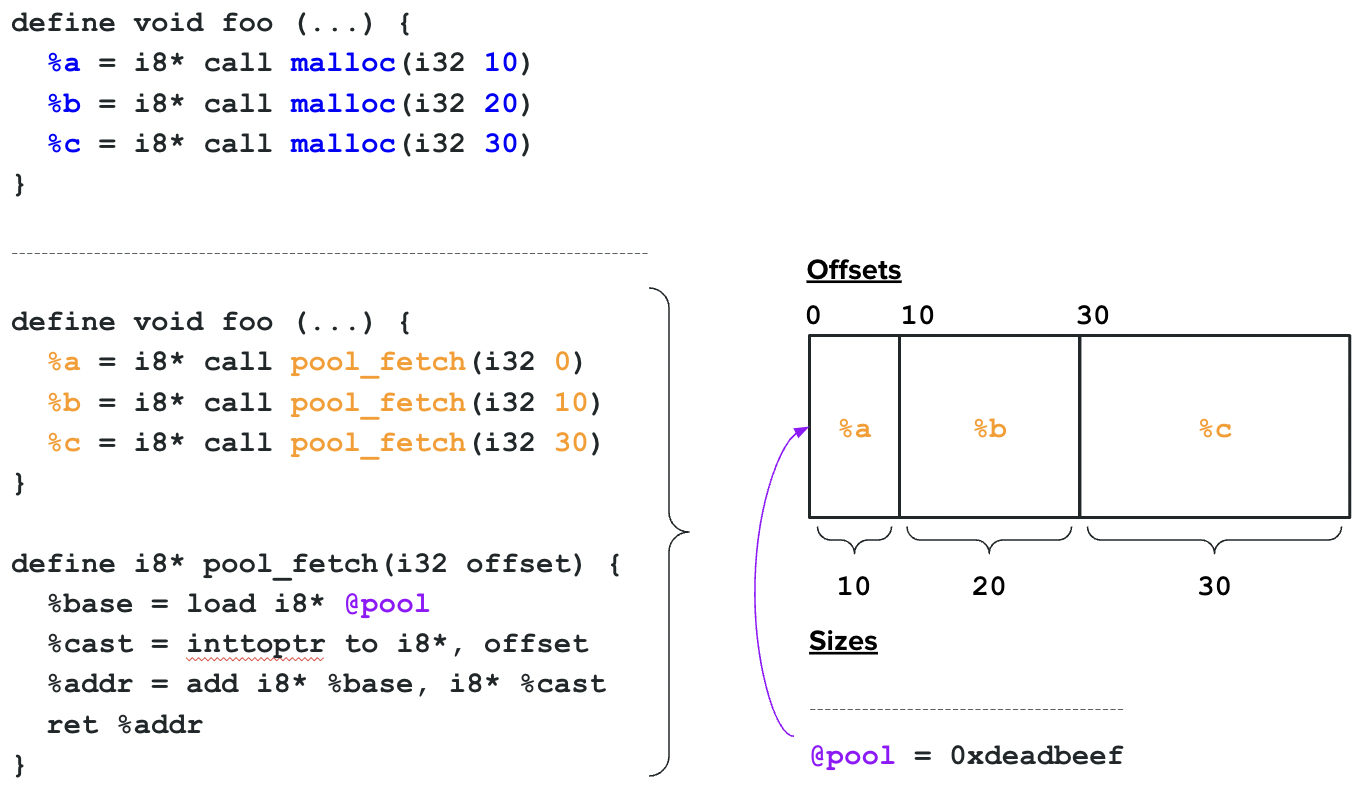
\includegraphics[width=0.77\textwidth]{figs/pool.png} 
        \caption{Example allocations (top) transformed to fetch from the compiler-directed
        memory pool (bottom; here, wrapped into the function \texttt{pool\_fetch}). The 
        basic functionality of the pool is shown to the right. In context of simplified LLVM 
        IR and \textit{libc} \texttt{malloc}.}  
	    \label{fig:pool}
\end{figure}

\section{Implementation}
The prototype compiler was built using LLVM 13.0.0. Both prototype runtimes (profiler and allocator) 
were implemented using \texttt{C++}. Profiler-guided compiler instrumentation for the custom 
allocator was not fully implemented and tested in this prototype due to its engineering effort.

In the allocator runtime in particular, bump allocators are organized in a red-black tree (\texttt{std::map})
where the key is the block size. Each bump allocator object allocates from an initial pool
containing (a default) 32 entries (each entry is sized to the block size). If there are no free entries
in the pool, another pool is allocated. Pools for a bump allocatore are also stored in a 
red-black tree (\texttt{std::map}), mostly to aid \DALLS .

Initialization for the compiler-directed memory pool and bump allocators (with known block size at 
compile-time) are injected by the compiler into a runtime function marked with the \texttt{constructor}
attribute. Although initialization is theoretically most performant when done in parallel
to FaaS startup, this was not implemented in the prototype.

Finally, all workloads are implemented in \texttt{C} and only use \textit{libc} \texttt{malloc} and 
\texttt{free}. Although most FaaS workloads are implemented in higher-level languages, the 
simplicity of the dynamic memory interface makes it very simple for the prototype compiler and 
runtime to target, as all \ALLS\ and \DALLS\ are obviously explicit. Targeting higher-level 
languages remains a future work. All inputs are placed on the stack as a simulation of the 
JIT/binary translation-based solution for embedding inputs into the binary before a FaaS 
instance executes.

The prototype can be found at \href{https://github.com/sgh185/849}{https://github.com/sgh185/849}.

\section{Evaluation}
To evaluate the prototype, four kernels (matrix multiplication, compressed-row-storage conversion,
breadth first traversal, and Huffman coding -- see Figure~\ref{fig:apps}) were used. All testing
was performed on a 28-Core Intel Xeon CPU E5-2690 v4 machine. All runs were single-threaded.  

\begin{figure}
        \small
        \centering
        \begin{tabular}{ | m{5cm} | m{7cm} | } 
          \hline
            Matrix Multiplication & Naive algorithm ; [60 x 30] x [30 x 120] \\ 
          \hline
            Compressed-Row-Storage (CSR) & Converts a [500 x 400] matrix to CSR form \\ 
          \hline
            Breadth First Traversal & Traversal on graph with 1000 vertices and records the traversal ; graph represented with adjancency matrix  \\ 
          \hline
            Huffman Coding & Builds a Huffman Tree for a block of "Lorem Ipsum" text \\ 
          \hline
        \end{tabular}
        \caption{Kernels used for evaluation.}
        \label{fig:apps}
\end{figure}

We assess the compiler transforms for the custom allocator both statically and dynamically. Figure~\ref{fig:static}
shows the number of eligible static \ALLS\ (\texttt{malloc}s column) in the baseline IR for each kernel and 
the number of \ALLS\ that were transformed to invoke the allocator ("Transformed" column). For matrix 
multiplication, the compiler aggressively unrolled the entire allocation loop for the result matrix
and inlined the entire \texttt{multiply} function. Consequently, all \SIZES\ were statically analyzable
and all \ALLS\ were transformed to fetch from the compiler-directed pool. For breadth first traversal and Huffman 
coding, almost all \ALLS\ were transformed to allocate from the bump allocator because most \ALLS\
were found in loops but had statically analyzable \SIZES . The \ALLS\ not transformed in
the Huffman coding kernel were all in functions that were inlined. The inlined static \ALLS\ were
all transformed.

\begin{figure}[htp]
    \centering
    \begin{minipage}{0.45\textwidth}
        \small
        \centering
        \begin{tabular}{ | m{5cm} | m{1cm} | m{2cm} | } 
          \hline
            Kernel & \texttt{malloc}s & Transformed \\
          \hline\hline
            Matrix Multiplication & 60 & 60 \\ 
          \hline
            Compressed-Row-Storage (CSR) & 3 & 0 \\ 
          \hline
            Breadth First Traversal & 7 & 7  \\ 
          \hline
            Huffman Coding & 17 & 10 \\ 
          \hline
        \end{tabular}
        \caption{Number of static allocations transformed.}
        \label{fig:static}
    \end{minipage}\hfill
    \begin{minipage}{0.45\textwidth}
        \centering
        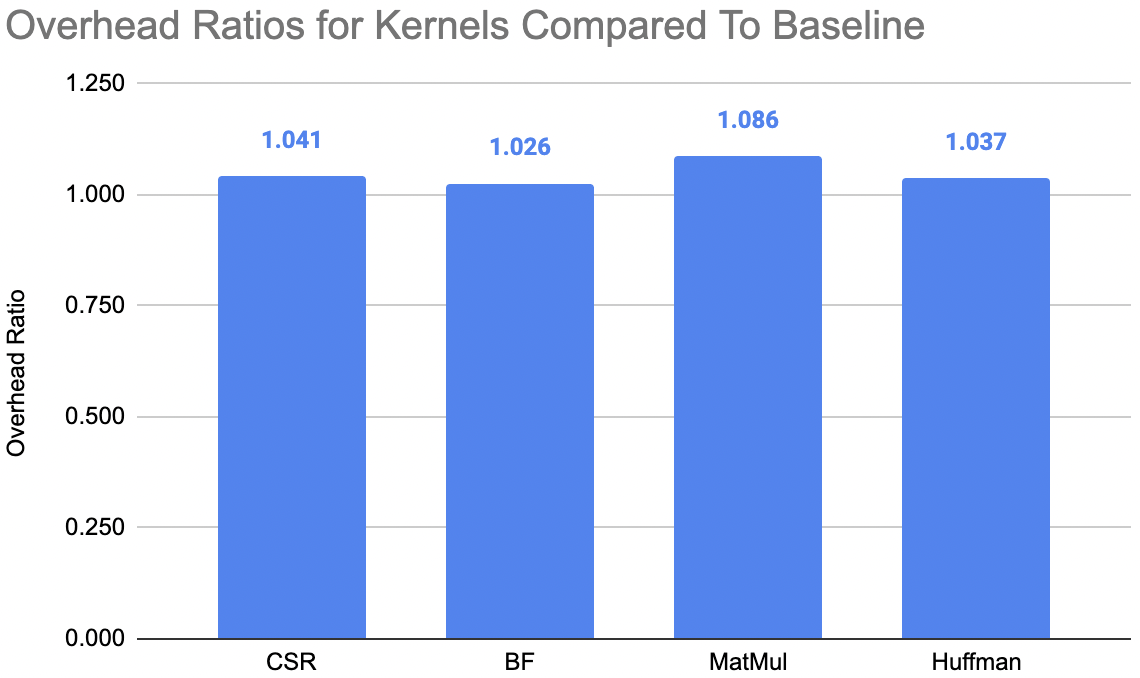
\includegraphics[width=0.88\textwidth]{figs/graph.png} 
        \caption{Overhead ratio for transformed kernels (with allocator runtime)
        vs. baseline kernels (no transform). Ratio compares cycle counts.}  
	    \label{fig:perf}
    \end{minipage}\hfill
\end{figure}

Next, we evaluate the performance of the transformed binaries against the baseline binaries (i.e.
without transformation, compiled straight from source code) for each kernel. Each kernel was 
run 10 times via \texttt{perf stat} and the cycle counts were recorded. Figure~\ref{fig:perf} shows the 
comparative overhead ratio (in terms of cycles). Here, all kernels have minimal overhead; although
matrix multiplication, in particular, should be faster. The lack of speedups could be attributed
to a very low-latency \texttt{malloc} coupled with extra initialization and runtime overhead. This
is explored in Figure~\ref{fig:cycles}. We break down the execution times for each major piece of the 
allocator runtime and highlight worst-case observed times (also in cycles). These overheads are
fairly substantial for the work that each method is performing. Some of the overhead can be due
to extra function calls because wrapper methods need to be exposed to the compiler for streamlined
instrumentation. Additionally, the data structures (\texttt{std::map}) used in the runtime and 
initialization costs may drive up overheads. Many of these overheads could be optimized by 
careful engineering.

\begin{figure} [htp]
        \small
        \centering
        \begin{tabular}{ | m{5cm} | m{9cm} | m{1cm} | } 
          \hline
            \texttt{Init} & Initialize the global allocator (that manages bump allocators) and compiler directed pool & 20418 \\ 
          \hline
            \texttt{AddAllocator} & Initialize a new bump allocator and add it to the global allocator & 27170 \\ 
          \hline
            \texttt{AllocateFromPool} & Fetching a pointer from the compiler-directed memory pool (wrapped as a function) & 52 \\ 
          \hline
            \texttt{AllocateFromBump} & Fetching a pointer from a bump allocator & 1372 \\ 
          \hline
            \texttt{AllocateFromBumpWithRuntimeInit} & Fetching a pointer from a bump allocator with allocator initialization, if necessary & 1372 \\ 
          \hline
        \end{tabular}
        \caption{Worst-case cycle times for essential methods in allocator runtime.}
        \label{fig:cycles}
\end{figure}

Note that the profiler, which outputs the \DWS\ and raw data on working set size 
every allocation/deallocation in the workload, is functional but not shown here. 

\section{Conclusion}
This paper shows a \crcd\ that analyzes and optimizes for dynamic memory usage in 
small FaaS workloads. The system provides a profiler, static allocation tracking and 
analysis, and a custom memory allocator controlled by both the compiler and runtime
tooptimize for dynamic memory. Across a small set of kernels, the compiler is 
successful at analyzing and transforming allocation candidates to use the custom
allocator, and the system achieves comparable performance compared to the baseline 
applications.

\bibliographystyle{plain}
\bibliography{sample}

\end{document}
